\documentclass[a4paper,12pt]{article} %размер бумаги устанавливаем А4, шрифт 12пунктов
\usepackage[T2A]{fontenc}
\usepackage[utf8]{inputenc}
\usepackage[english,russian]{babel} %используем русский и английский языки с переносами
\usepackage{amssymb,amsfonts,amsmath,mathtext,enumerate,float,amsthm} %подключаем нужные пакеты расширений
\usepackage[unicode,colorlinks=true,citecolor=black,linkcolor=black]{hyperref}
%\usepackage[pdftex,unicode,colorlinks=true,linkcolor=blue]{hyperref}
\usepackage{indentfirst} % включить отступ у первого абзаца
\usepackage[dvips]{graphicx} %хотим вставлять рисунки?
\graphicspath{{illustr/}}%путь к рисункам

\makeatletter
\renewcommand{\@biblabel}[1]{#1.} % Заменяем библиографию с квадратных скобок на точку:
\makeatother %Смысл этих трёх строчек мне непонятен, но поверим "Запискам дебианщика"

\usepackage{geometry} % Меняем поля страницы.
\geometry{left=2cm}% левое поле
\geometry{right=1cm}% правое поле
\geometry{top=2cm}% верхнее поле
\geometry{bottom=2cm}% нижнее поле

\renewcommand{\theenumi}{\arabic{enumi}}% Меняем везде перечисления на цифра.цифра
\renewcommand{\labelenumi}{\arabic{enumi}}% Меняем везде перечисления на цифра.цифра
\renewcommand{\theenumii}{.\arabic{enumii}}% Меняем везде перечисления на цифра.цифра
\renewcommand{\labelenumii}{\arabic{enumi}.\arabic{enumii}.}% Меняем везде перечисления на цифра.цифра
\renewcommand{\theenumiii}{.\arabic{enumiii}}% Меняем везде перечисления на цифра.цифра
\renewcommand{\labelenumiii}{\arabic{enumi}.\arabic{enumii}.\arabic{enumiii}.}% Меняем везде перечисления на цифра.цифра

\sloppy


%\renewcommand\normalsize{\fontsize{14}{25.2pt}\selectfont}

\usepackage[backend=biber,style=gost-numeric,sorting=none]{biblatex}
\addbibresource{all.bib}

% Пакет для отображения исходного кода - с http://www.inp.nsk.su/~baldin/LaTeX/lurs-code.pdf
\usepackage{listings}
%\usepackage{listingsutf8}
% подгружаемые языки — подробнее в документации listings
\lstloadlanguages{C++}
% Конфигурируем
\lstset{
	language=C++, % выбираем язык по умолчанию
	frame=single, % рамка
	commentstyle=\itshape\textcolor[rgb]{0.5,0.5,0.5}, % шрифт для комментариев
	stringstyle=\bfseries, % шрифт для строк
	numbers=left,              % где поставить нумерацию строк (слева\справа)
	numberstyle=\tiny,         % размер шрифта для номеров строк
	tabsize=2,                 % размер табуляции по умолчанию равен 2 пробелам
}

% А эта тёмная магия позволяет нормально работать с кириллицей в листингах
% Copyright Nikolay Avdeev aka NickKolok aka Николай Авдеев 2016

% Всем привет из снежного Воронежа!

% This file is part of LISTINGCYR.

%    LISTINGCYR is free software: you can redistribute it and/or modify
%    it under the terms of the GNU General Public License as published by
%    the Free Software Foundation, either version 3 of the License, or
%    (at your option) any later version.

%    LISTINGCYR is distributed in the hope that it will be useful,
%    but WITHOUT ANY WARRANTY; without even the implied warranty of
%    MERCHANTABILITY or FITNESS FOR A PARTICULAR PURPOSE.  See the
%    GNU General Public License for more details.

%    You should have received a copy of the GNU General Public License
%    along with CHAS-CORRECT.  If not, see <http://www.gnu.org/licenses/>.

%  (Этот файл — часть LISTINGCYR.

%   LISTINGCYR - свободная программа: вы можете перераспространять её и/или
%   изменять её на условиях Стандартной общественной лицензии GNU в том виде,
%   в каком она была опубликована Фондом свободного программного обеспечения;
%   либо версии 3 лицензии, либо (по вашему выбору) любой более поздней
%   версии.

%   LISTINGCYR распространяется в надежде, что она будет полезной,
%   но БЕЗО ВСЯКИХ ГАРАНТИЙ; даже без неявной гарантии ТОВАРНОГО ВИДА
%   или ПРИГОДНОСТИ ДЛЯ ОПРЕДЕЛЕННЫХ ЦЕЛЕЙ. Подробнее см. в Стандартной
%   общественной лицензии GNU.

%   Вы должны были получить копию Стандартной общественной лицензии GNU
%   вместе с этой программой. Если это не так, см.
%   <http://www.gnu.org/licenses/>.)
%





% Юзер, помни!
% Сей файл под GNU GPLv3.
% Слинковался - открой сорцы!
% Copyright Nikolay Avdeev 2016
% nickkolok@mail.ru or avdeev@math.vsu.ru

% Пользуясь случаем, передаю привет из Воронежа товарищу @virens

%Спасибо юзеру waverider за http://dxdy.ru/topic18924-15.html
\lstset{literate=
	{А}{{\CYRA}}1
	{Б}{{\CYRB}}1
	{В}{{\CYRV}}1
	{Г}{{\CYRG}}1
	{Д}{{\CYRD}}1
	{Е}{{\CYRE}}1
	{Ё}{{\CYRYO}}1
	{Ж}{{\CYRZH}}1
	{З}{{\CYRZ}}1
	{И}{{\CYRI}}1
	{Й}{{\CYRISHRT}}1
	{К}{{\CYRK}}1
	{Л}{{\CYRL}}1
	{М}{{\CYRM}}1
	{Н}{{\CYRN}}1
	{О}{{\CYRO}}1
	{П}{{\CYRP}}1
	{Р}{{\CYRR}}1
	{С}{{\CYRS}}1
	{Т}{{\CYRT}}1
	{У}{{\CYRU}}1
	{Ф}{{\CYRF}}1
	{Х}{{\CYRH}}1
	{Ц}{{\CYRC}}1
	{Ч}{{\CYRCH}}1
	{Ш}{{\CYRSH}}1
	{Щ}{{\CYRSHCH}}1
	{Ъ}{{\CYRHRDSN}}1
	{Ы}{{\CYRERY}}1
	{Ь}{{\CYRSFTSN}}1
	{Э}{{\CYREREV}}1
	{Ю}{{\CYRYU}}1
	{Я}{{\CYRYA}}1
	{а}{{\cyra}}1
	{б}{{\cyrb}}1
	{в}{{\cyrv}}1
	{г}{{\cyrg}}1
	{д}{{\cyrd}}1
	{е}{{\cyre}}1
	{ё}{{\cyryo}}1
	{ж}{{\cyrzh}}1
	{з}{{\cyrz}}1
	{и}{{\cyri}}1
	{й}{{\cyrishrt}}1
	{к}{{\cyrk}}1
	{л}{{\cyrl}}1
	{м}{{\cyrm}}1
	{н}{{\cyrn}}1
	{о}{{\cyro}}1
	{п}{{\cyrp}}1
	{р}{{\cyrr}}1
	{с}{{\cyrs}}1
	{т}{{\cyrt}}1
	{у}{{\cyru}}1
	{ф}{{\cyrf}}1
	{х}{{\cyrh}}1
	{ц}{{\cyrc}}1
	{ч}{{\cyrch}}1
	{ш}{{\cyrsh}}1
	{щ}{{\cyrshch}}1
	{ъ}{{\cyrhrdsn}}1
	{ы}{{\cyrery}}1
	{ь}{{\cyrsftsn}}1
	{э}{{\cyrerev}}1
	{ю}{{\cyryu}}1
	{я}{{\cyrya}}1
}

% Люди, любите друг друга, используйте Linux и поступайте на матфак ВГУ!








\begin{document}

\setcounter{page}{2}

\section*{Предварительные сведения}

В качестве основного пособия по языку C++ используется \cite{chmyhalo}.


Блок-схемы выполняются в соответствии с \cite{gost-block-scheme};
ряд примеров имеется в \cite{wiki-block-scheme}.


\section*{Постановка задачи}
Составить алгоритм и написать программу
для возведения длинного целого числа в длинную натуральную степень.

Составить алгоритм и написать программу
для деления двух длинных целых чисел с остатком.

\section*{Организация работы с длинными числами}

Возведение в степень выполняется не циклическим умножением,
а чередующимися умножением и возведением в квадрат \cite{Glukhov}.
Так как основание степени подвергается мультипликативным операциям,
то оно записывается в $10^4$--чной системе счисления.
С показателем степени ситуация несколько иная:
деление на 2 с остатком, вообще говоря,
не обязательно проводить в той же системе счисления, в которой записано основание;
из соображений экономии выбрана $10^9$--чная система,
поскльку максимальное число, получаемое в результате сноса разряда,
в таком случае не превышает $2\cdot 10^9 - 1$,
что укладывается в ограничения 32-битных целых.

Деление на 2 в целях экономии времени реализуется <<на месте>>,
т.е. частное пишется на место делимого, остаток возвращается.

Деление выполняется по алгоритму, предложенному Глуховым \cite{Glukhov};
делитель и делимое должны быть записаны в одинаковой системе счисления;
поскольку делимое подвергается мультипликативным операциям,
то и для делимого, и для делителя используется $10^4$--чная система счисления.

При делении числа считаются положительными,
поскольку учёт знака не представляет алгоритмического интереса.

Имевшиеся функции сравнения и вычитания разделены на две части:
первая часть каждой функции, сохранившая название,
используется для работы с объектами класса BigInt
и принимает только два аргумента
(вся сопутствующая информация: основание системы счисления, длина числа~--- инкапсулированы).
Вторая же часть работает с указателями и, кроме них, принимает все необходимые параметры.


\section*{Исходный код программы}

\lstinputlisting[caption={class\_int.cpp}]{../class_int.cpp}
\lstinputlisting[caption={class\_int\_square.cpp}]{../class_int_square.cpp}
\lstinputlisting[label=BigIntClass,caption={class\_int\_division.cpp}]{../class_int_division.cpp}
\lstinputlisting[label=BigIntClass,caption={class\_int\_roots.cpp}]{../class_int_roots.cpp}
\lstinputlisting[label=Summing,caption={square\_root.cpp}]{../square_root.cpp}

\section*{Блок-схемы}

Блок-схемы приводятcя только для подалгоритмов, представляющих интерес с точки зрения реализации работы с длинными числами,
а именно нормализации по Глухову, деления с остатком по Глухову,
деления с остатком на 2, возведения в степень.
Алгоритмически тривиальные конструкции --- наподобие перегрузки операторов потока или индекса --- на блок-схемах не отражаются,
дабы избежать загромождения отчёта.


\begin{figure}[ht]
	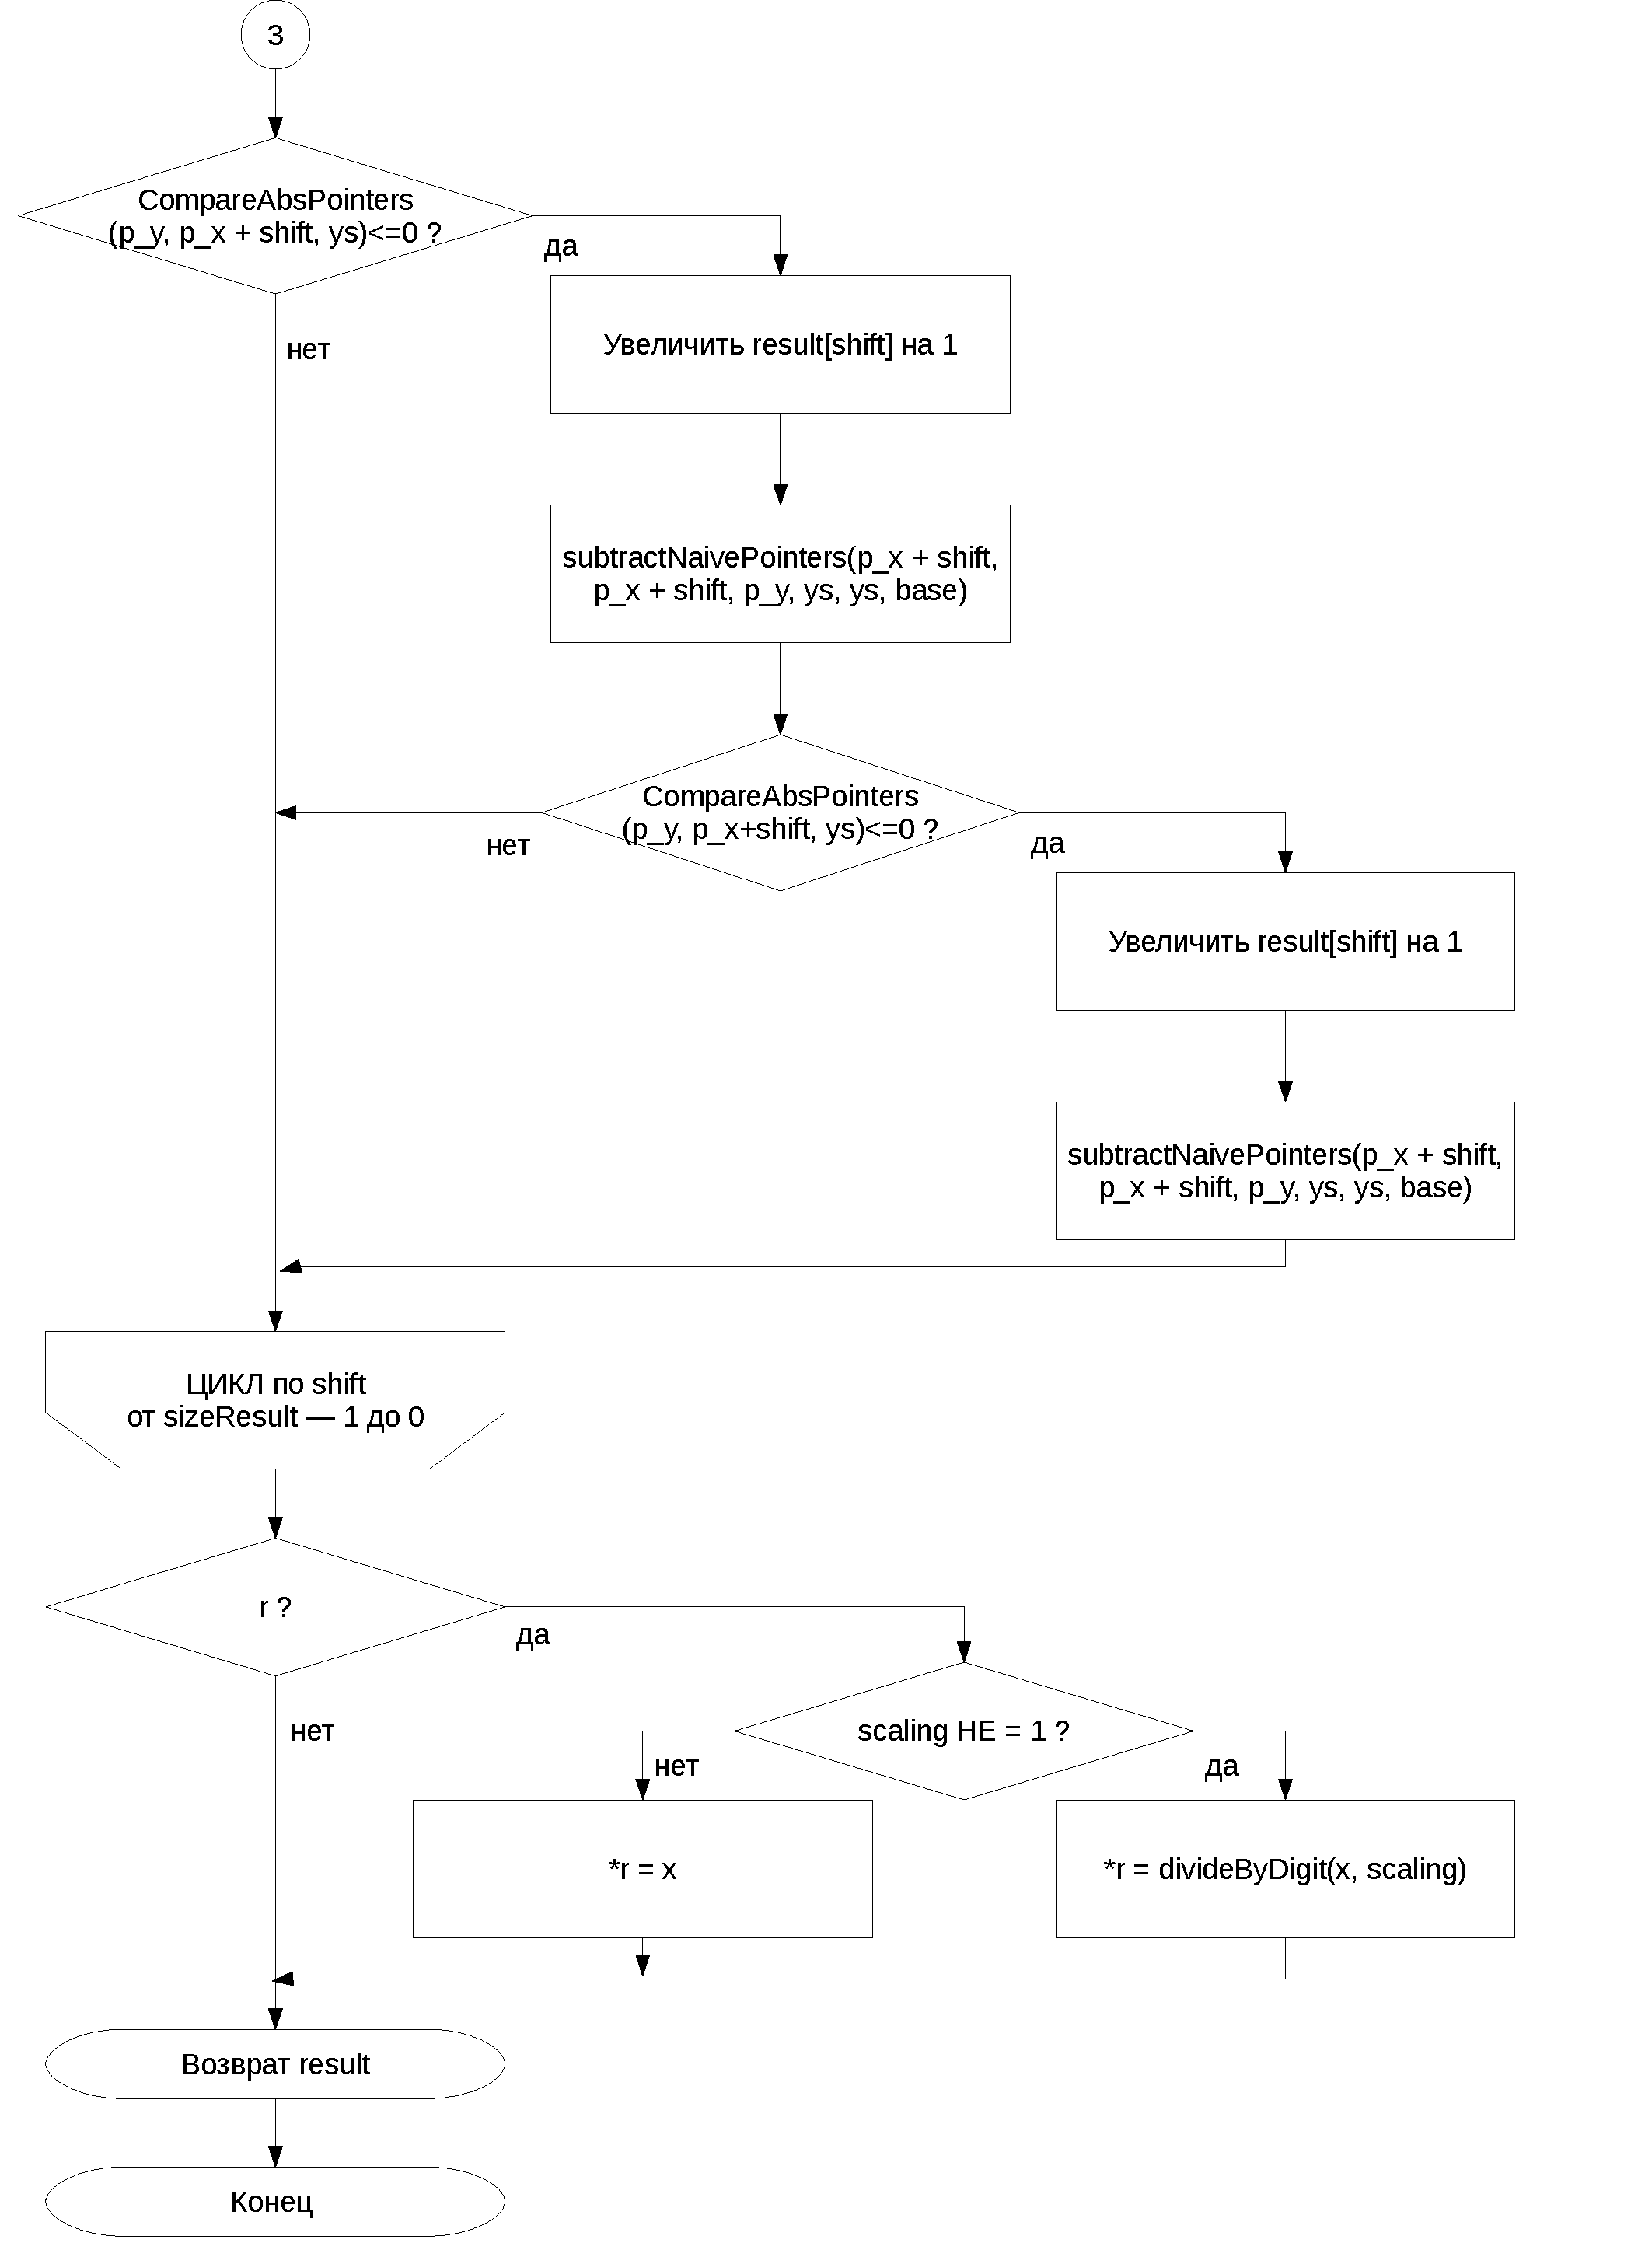
\includegraphics[width=\textwidth]{lr3_divide-3.pdf}
	\caption{Блок-схема алгоритма деления по Глухову: функция BigInt divide(BigInt x, BigInt y, BigInt* r)}
\end{figure}


\clearpage

\section*{Результаты работы программы}



\subsection*{Возведение в степень (запуск 1)}
\begin{verbatim}
(program exited with code: 0)
Press return to continue
\end{verbatim}

\printbibliography
\end{document}
